\documentclass[]{manual}

\title{Fourier Optics}
\date{\today}
\course{Physics 325}

\begin{document}
    \maketitle
    \thispagestyle{firstpage}

    %%%

    \section{Motivation}

    One of the most beautiful results in optics is that far-field diffraction is essentially a Fourier transform of the diffracting object.
    In this lab we will explore this idea by building a Fourier imaging system from scratch and using it to gain some intuition about far-field diffraction.

    \section{Background}

    Imagine that we have some aperture of width $W$ with an assortment of opaque blockages in it.
    What is the image in the far field when an electromagnetic wave is incident on the aperture from the left, as shown in Figure~\ref{fig:single-slit-diffraction-geometry}?

    \begin{figure}
        \centering

        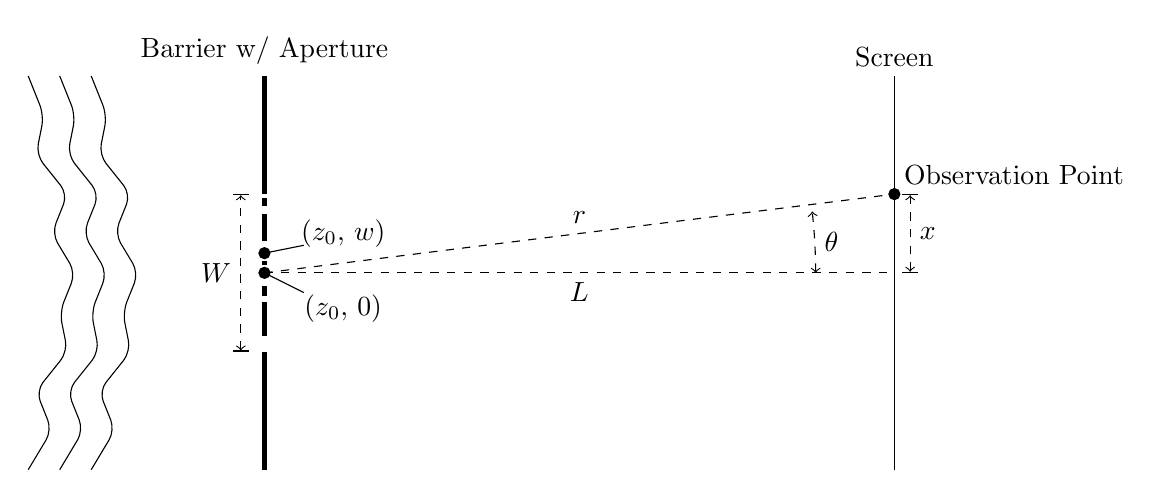
\begin{tikzpicture}
            \foreach \x in {0, .4, .8}
                \draw[rounded corners] (-3 + \x, 5)
                 -- (-2.8 + \x, 4.5)
                 -- (-2.9 + \x, 4)
                 -- (-2.5 + \x, 3.5)
                 -- (-2.7 + \x, 3)
                 -- (-2.4 + \x, 2.5)
                 -- (-2.6 + \x, 2)
                 -- (-2.5 + \x, 1.5)
                 -- (-2.9 + \x, 1)
                 -- (-2.7 + \x, 0.5)
                 -- (-3 + \x, 0);

            \draw[|<->|, dashed] (-0.3, 1.5) -- (-0.3, 3.5) node[midway, left] {$W$};

            \draw[ultra thick] (0, 0) -- (0, 1.5);
            \draw[ultra thick] (0, 3.5) -- (0, 5) node[above] {Barrier w/ Aperture};
            \draw[ultra thick] (0, 1.7) -- (0, 2.13);
            \draw[ultra thick] (0, 2.2) -- (0, 2.33);
            \draw[ultra thick] (0, 2.6) -- (0, 2.65);
            \draw[ultra thick] (0, 2.9) -- (0, 3.25);
            \draw[ultra thick] (0, 3.35) -- (0, 3.45);

            \draw[dashed] (0, 2.5) -- (8, 2.5) node[midway, below] {$L$};

            \draw[dashed] (0 ,2.5) -- (8, 3.5) node[midway, above] {$r$};

            \draw[|<->|, dashed] (8.2, 2.5) -- (8.2,3.5) node[midway, right] {$x$};

            \draw[<->, dashed] (7, 2.5) arc (0:6.4:7) node[midway, right] {$\theta$};

            \draw[fill] (0, 2.5) circle (2pt);
            \draw (0, 2.5) -- (0.5, 2.25);
            \node[align=center,below] at (1,2.35) {$(z_0, \, 0)$};

            \draw[fill] (0, 2.75) circle (2pt);
            \draw (0, 2.75) -- (0.5, 2.85);
            \node[align=center,above] at (1,2.7) {$(z_0, \, w)$};

            \draw (8, 0) -- ++(0, 5) node[above] {Screen};

            \draw[fill] (8,3.5) circle (2pt) node[above right] {Observation Point};
        \end{tikzpicture}

        \caption{An electromagnetic wave illuminating an arbitrary aperture.}

        \label{fig:single-slit-diffraction-geometry}
    \end{figure}
    
    To determine what we see on the screen (i.e., $I(x) = \abs{E(x)}^2 = E(x) \, E^*(x)$, called the ``intensity pattern'' or ``diffraction pattern''), we will use \textbf{Huygen's Principle}, which says that we can treat each point in the aperture as an independent spherical emitter.
    To determine the electric field anywhere, we sum over the contributions from each point:
    \begin{align}
    E(z, x) &= \int^{W/2}_{-W/2} \dd{w} E(z_0, w) \, \frac{e^{i k r}}{r} = \int^{W/2}_{-W/2} \dd{w} E(z_0, w) \, \frac{e^{i k \sqrt{(w-x)^2 + L^2}}}{\sqrt{(w-x)^2 + L^2}},
    \end{align}
    where $z$ is the coordinate going between the barrier and the screen, $x$ is the distance along the screen to the observed point, $r$ is the distance from some point in the aperture to the observed point on the screen, $w$ is the distance of that point to the center of the aperture, $W$ is the width of the aperture, and $k = 2 \pi / \lambda$ is the wavenumber of the light.  
    
    This integral is not tractable without making some assumptions.
    We will assume that we are in the \textbf{far-field}: $L \gg W$.
    This type of diffraction is called \textbf{Fraunhofer diffraction}.
    We can now approximate the square root in the exponent as
    \begin{align} \label{eqn:fraunhoffer-square-root-approx}
    \sqrt{(s-x)^2 + L^2} = \sqrt{w^2 + x^2 - 2wx + L^2} = r \, \sqrt{1 + \frac{-2wx + w^2}{r^2}} \approx r \qty(1 - \frac{wx}{r^2}),
    \end{align}
    and the square root in the denominator as $\sqrt{(w-x)^2 + L^2} = r$. 
    Now we have
    \begin{align} \label{eqn:fraunhofer-diffraction-integral}
    E(x) &= \frac{e^{i k r}}{r} \, \int^{W/2}_{-W/2} \dd{w} E(z_0, w) \, e^{-i k \frac{x}{r} w}.
    \end{align}
    The integral in the above equation accounts for the interference of all the point sources in the aperture, each with initial amplitude $E(z_0, w)$, at point $x$ on the screen.  The phase factor outside the integral is common to all the point sources and accounts for the phase accumulated from propagating the distance $r$ from the aperture to the screen. Note that $E(z_0, w)=0$ whenever $w$ coincides with one of the blockages.

    It turns out that we can capture the behavior of this integral in a much more intuitive way.
    Let's return to Eq.~\eqref{eqn:fraunhofer-diffraction-integral} and rewrite the exponential phase factor using $x / r = \sin \theta$.
    If we think of $E(z_0, w)$ as containing the information about the slit restricting the electric field (so that we can relax the bounds on the integral), we have
    \begin{align}
        E(x) &= \frac{e^{i \kappa r}}{r} \, \int^{\infty}_{-\infty} \dd{w} E(z_0, w) \, e^{-i k \sin\theta \, w} \nonumber \\
        E(x) &= \frac{e^{i \kappa r}}{r} \, \int^{\infty}_{-\infty} \dd{w} E(z_0, w) \, e^{-i \kappa \, w}.
    \end{align}
    That's a Fourier transform!
    The transform variable $\kappa = k \sin{\theta}$ is the \textbf{transverse spatial frequency} (transverse being perpendicular to the propagation direction of the light).
    Apparently, diffracting off of an obstructing object produces a far-field image based on the amplitudes of the different \textbf{spatial frequency components} of the obstructing object's transverse features.
    Spatial frequency has units of inverse length, just like time-based frequency has units of inverse time.

    This agrees with what we learned (or will learn) in the Diffraction lab by doing the integral manually, because the Fourier transform of a rectangle is a $\sinc$ function.
    When we shone light on a rectangular slit the intensity pattern we observed was $\sinc^2$, so the underlying electric field must have been a $\sinc$.
    Thinking about far-field diffraction using the Fourier transform is a specialty sub-field all it's own: \textbf{Fourier optics}.

    In this lab we will build a Fourier imaging setup from scratch.
    The schematic of the setup is shown in Figure~\ref{fig:fourier-optics-setup}.
    The spatial filter (containing a thin lens and a pinhole) cleans up the input beam.
    The resulting beam, which will be expanding rapidly since it just went through a tiny aperture (can you explain why in terms of Fourier optics?) is sent through a thick lens to bring it back under control.
    The beam then passes through the object, which acts just like the slits we have been using up until now (except, of course, that the pattern is more complicated).
    The achromatic lens pulls the far-field into the near-field, placing it on the lower prism's upper surface.

    At this point the intensity pattern is the Fourier transform of the object, and we will in fact be able to see it on the surface of the prism.
    But, we just produced an object in the new near-field, so if we let the beam keep propagating, we can eventually get it to Fourier transform \textbf{again}.
    The doubly-Fourier-transformed image is picked up using the mirror and screen after the prism pair.
    This is an interesting addition to the setup: we can modify the Fourier transform in the near-field and see the results in the far-field.

    \begin{figure}
        \centering

        \begin{tikzpicture}[optics/.style={thick,fill=gray!30}]
            \pgfmathsetmacro{\h}{1.5}

            % laser
            \draw[optics] (0, 0) rectangle (2, \h) node[midway] {Laser};
            
            % spatial filter
            \pgfmathsetmacro{\filterx}{2.8}
            \pgfmathsetmacro{\filterlength}{2}
            \pgfmathsetmacro{\filterheight}{1.1*\h}
            \draw[optics] (\filterx, {(\h-\filterheight)/2}) rectangle ++(\filterlength, \filterheight);
            \node[above] at (\filterx + \filterlength/2, \h) {Spatial Filter}; 

            % thin lens
            \pgfmathsetmacro{\thinlensx}{3}
            \pgfmathsetmacro{\r}{3}
            \pgfmathsetmacro{\startAngle}{asin(\h/\r)/2}
            \draw[optics] (\thinlensx, \h)
            arc[start angle=180-\startAngle,delta angle=2*\startAngle,radius=\r]
            arc[start angle=-\startAngle,delta angle=2*\startAngle,radius=\r]
            -- cycle;

            % pinhole
            \pgfmathsetmacro{\pinholex}{4.05}
            \draw[ultra thick] (\pinholex, -.05*\h) -- (\pinholex, {(\h/2)-.1});
            \draw[ultra thick] (\pinholex, {(\h/2)+.1}) -- (\pinholex, 1.05*\h);

            % thick lens
            \pgfmathsetmacro{\thicklensx}{6.5}
            \draw[optics] (\thicklensx, \h) -- ++(0, -\h)
            -- ++(-.5, 0)
            .. controls (\thicklensx-0.8, \h/3) and (\thicklensx-0.8, 2*\h/3) .. ++(0, \h)
            node[pos=.3, inner sep=0pt] (thicklower) {}
            node[pos=.7, inner sep=0pt] (thickupper) {}
            -- cycle;
            \node[above] at ({\thicklensx}, \h) {Thick Lens};

            % object
            \foreach \x in {0,.1,...,.5} {
                \draw[thin] ({8+\x},{0-(\x/2)+(\h/4)}) -- ++({\h/3}, {\h/2+0.2});
            }
            \node[above] at (8.5, \h) {Object};

            % achromat
            \pgfmathsetmacro{\achromatx}{9.5}
            \pgfmathsetmacro{\r}{3}
            \pgfmathsetmacro{\startAngle}{asin(\h/\r)/2}
            \draw[optics] (\achromatx, \h)
            arc[start angle=180-\startAngle,delta angle=2*\startAngle,radius=\r]
            arc[start angle=-\startAngle,delta angle=2*\startAngle,radius=\r]
            -- cycle;
            \node[below] at (\achromatx, 0) {Achromatic Lens};

            % prism pair
            \pgfmathsetmacro{\prismx}{11}
            \draw[optics] (\prismx, \h) -- ++(0, -\h) -- ++(\h, \h)
            node[pos=.5, inner sep=0pt] (prismlower1) {}
            node[pos=.6, inner sep=0pt] (prismlower2) {}
            -- cycle
            node[pos=0.4, inner sep=0pt] (prismlowerjoin) {}
            ;
            \draw[optics] (\prismx, 1 + \h) -- ++(0, \h) -- ++(\h, -\h)
            node[pos=0.5, inner sep=0pt] (prismupper) {}
            -- cycle;
            \node[above right] at (\prismx, {(2*\h)+1}) {Prism Pair};
            \draw[<-, dashed, shorten <=.1cm] (prismlowerjoin) -- ++(.6, .5) node[right, inner sep=0pt] {$\mathcal{F}\qty{\mathrm{Object}}$};

            % mirror
            \draw[fill] (1, 3) rectangle ++(.1, 1) node[midway, inner sep=0pt] (mirror) {};
            \node[below] at (1.05, 3) {Mirror};

            % screen
            \draw[fill] (8, 4) rectangle ++(.1, 1) node[midway, inner sep=0pt] (screen) {};
            \node[above] at (8.05, 5) {Screen};
            \draw[<-, dashed, shorten <=.1cm] (screen) -- ++(-.8, .5) node[left, inner sep=0pt] {$\mathcal{F}\qty{\mathcal{F}\qty{\mathrm{Object}}}$};

            % upper beam
            \pgfmathsetmacro{\upper}{2*\h/3}
            \pgfmathsetmacro{\lower}{\h/3}

            \draw[neararrow={stealth}] (2, \upper) -- (\thinlensx, \upper) -- (thicklower);
            \draw[dotted] (thicklower) -- (\thicklensx, \lower);
            \draw[midarrow={stealth}] (\thicklensx, \lower) -- (\achromatx, \lower);
            \draw (\achromatx, \lower) -- (prismlower1) -- (prismlowerjoin) -- (prismupper);

            % lower beam
            \draw[neararrow={stealth}] (2, \lower) -- (\thinlensx, \lower) -- (thickupper);
            \draw[dotted] (thickupper) -- (\thicklensx, \upper);
            \draw[midarrow={stealth}] (\thicklensx, \upper) -- (\achromatx, \upper);
            \draw (\achromatx, \upper) -- (prismlower2) -- (prismlowerjoin) -- (prismupper);

            % combined beam
            \draw[midarrow={stealth}] (prismupper) -- (mirror);
            \draw[midarrow={stealth}] (mirror) -- (screen);
        \end{tikzpicture}

        \caption{The Fourier optics setup.}

        \label{fig:fourier-optics-setup}
    \end{figure}

    You may find the Fourier transform identities and properties listed in Table~\ref{tab:fourier-transform-properties} helpful.

    \begin{table}
        \centering

        \renewcommand{\arraystretch}{1.5}
        \begin{tabular}{ c c c }
            Function & Fourier Transform & Name \\
            \hline
            $a \, f(x) + b \, g(x)$ & $a \, \hat{f}(\kappa) + b \, \hat{g}(\kappa)$ & Linearity \\
            $f(c x)$ & $\frac{1}{c} \hat{f}(\frac{\kappa}{c})$ & Scaling \\
            $f(x - c)$ & $\hat{f}(\kappa) \, e^{-i \, 2 \pi \, a \kappa}$ & Shift \\
            $f(x) * g(x)$ & $\frac{1}{\sqrt{2 \pi}} \hat{f}(\kappa) \, \hat{g}(\kappa)$ & Convolution Theorem \\
            $e^{i k_0 \kappa}$ & $\sqrt{2 \pi} \, \delta(\kappa - \kappa_0)$ & Delta Function \\
        \end{tabular}
        \renewcommand{\arraystretch}{1}

        \caption{
            A few particularly useful identities involving the Fourier transform.
            The convolution of $f$ and $g$ is defined to be $f * g = \int_{-\infty}^{\infty} \dd{\sigma} f(x) g(x - \sigma)$.
            Due to the duality of the Fourier transform (the Fourier transformation is its own inverse), all of these properties are true in reverse as well.
            For example, the Fourier transform of a product of two functions is the convolution of their Fourier transforms.
        }

        \label{tab:fourier-transform-properties}
    \end{table}


    \section{Equipment}

    For this lab, you will need:
    \begin{itemize}
        \item The pieces of the Fourier imaging setup, with mounts for each:
        \begin{itemize}
            \item A Helium-Neon (He-Ne) laser.
            \item A spatial filter (with internal lens and pinhole).
            \item A thick converging lens.
            \item An achromatic lens.
            \item A right-angle prism pair.
            \item A mirror.
            \item A screen.
        \end{itemize}
        \item Various masks, to block out portions of the Fourier transform.
        \item Various ``objects'', like wire grids and circular holes.
        \item A diffuser, to make it easier to view the Fourier transform on the prism surface.
    \end{itemize}

    \FloatBarrier
    \newpage

    \section{Procedure}

    \FloatBarrier

    \subsection{Thinking Fourier}
    
    One of the most straightforward applications of the ideas of Fourier optics is to predict what light will look like after passing through an aperture without grinding through integrals.

    \checkpoint{
        Make a \textbf{qualitative} prediction about what the Fourier transform of each of the four objects shown in Figure~\ref{fig:fourier-objects} will look like based on the ideas of Fourier optics.
    }

    \begin{figure}
        \centering

        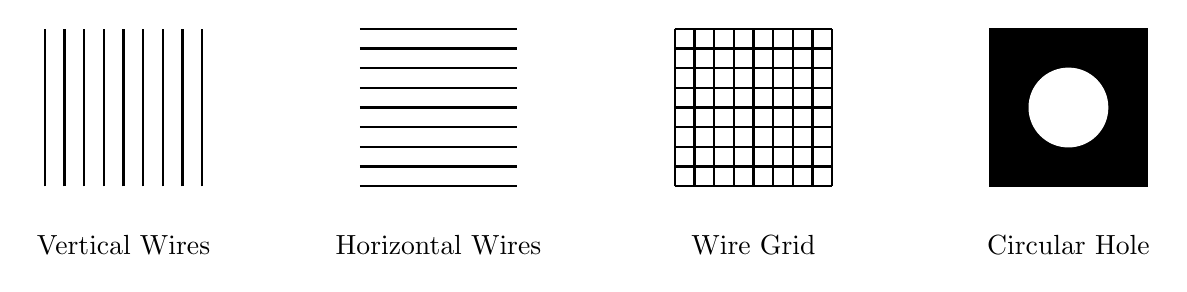
\begin{tikzpicture}
            \node[below] (verticalwires) at (0, 0) {Vertical Wires};
            \node[below] (horizontalwires) at (4, 0) {Horizontal Wires};
            \node[below] (grid) at (8, 0) {Wire Grid};
            \node[below] (hole) at (12, 0) {Circular Hole};

            % vertical
            \foreach \x in {-1,-.75,...,1}
                \draw[thick] (\x, .5) -- (\x, 2.5);

            % horizontal
            \foreach \y in {.5,.75,...,2.5}
                \draw[thick] (3, \y) -- (5, \y);

            % grid
            \foreach \y in {.5,.75,...,2.5}
                \draw[thick] (7, \y) -- (9, \y);
            \foreach \x in {7,7.25,...,9}
                \draw[thick] (\x, .5) -- (\x, 2.5);

            % hole
            \draw[fill] (11, .5) rectangle (13, 2.5);
            \draw[fill, color=white] (12, 1.5) circle[radius=.5];

        \end{tikzpicture}

        \caption{Objects to Fourier transform.}

        \label{fig:fourier-objects}
    \end{figure}

    \subsection{Building the Fourier Imaging System}

    Here is the alignment procedure for the setup:
    \begin{enumerate}
        \item Set up everything except the lenses.
        Align the laser beam through the optical setup so that it hits (roughly) the centers of the prisms, the mirror, and the screen.
        \item Add the spatial filter, ensuring that the pinhole is on the side of the device away from the laser.
        Adjust it until you get a clean, bright, rapidly-diverging bullseye pattern coming through the filter.
        \item Add the thick lens (large side away from the laser) and adjust its position to produce a collimated beam that still passes roughly through the center of the rest of the optical elements.
        \item Add the achromatic lens to the system, and move it so that its focal plane is the exit surface of the first prism.
        \item Install the wire grid object.
        You should see its Fourier transform on the exit surface of the first prism in sharp focus - adjust the achromatic lens until this is so.
        You should also be able to see the Fourier transform \textit{of the Fourier transform} (i.e., the original object) on the screen.
        Again, adjust until this is so.
    \end{enumerate}

    \checkpoint{
        Construct and align the Fourier imaging system.
        \begin{itemize}
            \item Check your predictions from the previous checkpoint by using the masks.
        \end{itemize}
    }

    \subsection{The Wild World of Fourier Transforms}

    We will now investigate some of the strange things we can make happen by interacting with the Fourier transform of the object.
    Remember that although we can only see the intensity of the light in the Fourier transform, the phase of the light matters as well.
    Changing either of them will change what we see on the screen.

    Install the wire grid object.

    \checkpoint{
        Mask out all but a single row or column of dots.
        \begin{itemize}
            \item What do you see on the screen? Why?
        \end{itemize}
    }

    \checkpoint{
        Mask out all but the central dot.
        What do you see on the screen?
        \begin{itemize}
            \item This mask is a \textbf{spatial frequency filter}.
                  Is it a high-pass filter (lets through high frequencies, blocks low frequencies), a low-pass filter (lets through low frequencies, blocks high frequencies), or a notch filter (blocks a certain range of frequencies)?
        \end{itemize}
    }
    
    Carefully install the glass chip phase-shifter over the central dot, so that the light of just that frequency component passes through the glass chip, while as many other frequency components as possible are unperturbed.

    \checkpoint{
        Rotate the chip to change the phase of that frequency component.
        
        \begin{itemize}
            \item What happens to the image?
            \item Which property from Table~\ref{tab:fourier-transform-properties} describes what is happening?
        \end{itemize}
    }

    Install the circular hole object.

    \checkpoint{
        Move the hole around, and note that the Fourier transform (called an ``Airy disk'') does not appear to change shape or position.
        However, the image on the screen will still move with the physical object!
        How is the information about the position of the object being stored in the traveling light?
    }

    \newpage
    \FloatBarrier

    \section{Prelab Questions}
    \setcounter{subsection}{0}

    \subsection*{A Fourier Transform}

    Show that the Fourier transform of the centered rectangle function is a $\sinc$ function ($\sinc(y) \equiv \sin(y)/y$).
    The centered rectangle function of width $a$ is
    \begin{align*}
        R_a(x) &= \begin{cases}
            1 & \abs{x} \leq a/2 \\
            0 & \mathrm{otherwise}
        \end{cases}
    \end{align*}
    and the normalized Fourier transform of a function $f(x)$ is $\mathcal{F}\qty{f(x)}(\kappa) \equiv \hat{f}(\kappa)$, defined to be
    \begin{align*}
        \hat{f}(\kappa) &= \frac{1}{\sqrt{2\pi}} \int \dd{x} f(x) \, e^{-i \kappa x}.
    \end{align*}

\end{document}
